\chapter{测试与结果分析}

\section{实验设置}
实验分别考察完整系统的运行成本、三项主要优化、部署改动和功能正确性。数学基础见第二章，
具体算法与参数见第四章；身份和消息采用规范字节编码，正常密码操作使用操作系统随机源。十种
常规组合的主比较全部采用表~\ref{tab:environments}中的统一环境，专项实验环境在相应小节另列。

\begin{table}[H]
\centering\small
\caption{十种常规组合的同机实验环境与方法}
\label{tab:environments}
\begin{tabularx}{\textwidth}{@{}p{.24\textwidth}X@{}}
\toprule
\rowcolor{black!8} 项目 & 统一条件 \\
\midrule
硬件与系统 & Intel Core Ultra 9 275HX；WSL2 Linux；固定逻辑CPU 0--3 \\
运行时与线程 & Sage 10.9、Python 3.13.14；OMP 4，OpenBLAS、MKL与NUMEXPR均为1线程 \\
输入 & 发送与接收身份各64 B，应用消息32 B，系统随机源 \\
重复方式 & 每种组合建立1个独立根；首次、同进程重复和新进程恢复后操作各1次 \\
记录项目 & 各阶段墙钟时间、规范对象与完整密文字节数、进程树采样RSS、诚实结果与外层拒绝 \\
\bottomrule
\end{tabularx}
\end{table}

完整流程计时包含组合编码、对象检查和原语调用。首次解密包含叶钥生成；恢复实验另起进程加载
已有对象。十种组合的实验固定逻辑CPU~0--3，OpenBLAS、MKL与NUMEXPR均为1线程，首次操作在运行库
准备后开始计时。表中重复测量描述固定密钥下的运行波动，独立建立系统的数量单独列出。下文时间
通常保留3位有效数字；B、KiB、MiB分别表示字节、$2^{10}$字节和$2^{20}$字节。

\subsection{组合覆盖与代表方案}

第四章表~\ref{tab:implemented-matrix}已经列出两种HIBE与五种常规IBS形成的十种组合。测试阶段
对每一格都调用真实后端，完成系统建立、双方发钥、首次与重复消息收发、新进程恢复和外层篡改
拒绝。组合数量按底层算法计数，同一算法的不同参数档及参考／紧凑格式不重复计为新方案。

十种组合形成常规后端的主要横向比较；A、B、C在此基础上承担更深入的重复、阶段分解和专项优化
分析。Wang--PW是在常规十种组合之后接入的第六种IBS，目前完成LATTE＋Wang--PW目标档，
其输入长度、运行机器和资源规模不同，因而以独立的分阶段结果呈现。

\subsection{评价指标}

实验按“离线准备、在线收发、持久恢复”三阶段记录。离线准备包括系统建立与双方发钥；在线
收发包括首次加密、首次解密和固定密钥下的重复操作；持久恢复另起进程加载公开对象与角色密钥。
时间采用墙钟时间，尺寸采用实际规范编码字节数，内存采用定期采样的进程树RSS峰值。

这些指标对应不同部署选择。发钥机构更关心Setup、KeyExtract和主状态，发送端更关心签名与
完整加密，接收端更关心叶钥委派和解密，网络侧则关心完整密文而不是单个签名。后文先分析
完整系统，再把总成本分解到具体优化。

\section{十种常规组合的同机基本比较}

\subsection{实验方法与完成情况}

十种组合使用同一份固定源码归档、相同原生引擎和依赖版本，按串行方式运行。三组来自同口径
预运行，另外七组在相同环境下补齐；两批的源码摘要、软件环境、线程设置和输入完全一致。每种
组合建立一套独立系统及主密钥，依次执行首次加解密、同进程重复加解密、新进程对象恢复和恢复后
解密，并分别检查密文截断和单比特翻转。

十种组合全部完成，共通过20次诚实加密、30次诚实解密、10次新进程恢复和20次外层拒绝，没有
失败记录。每项时间为一个独立根上的一次实测。所用配置均为第四章列出的目标或论文参数而非教学
参数；哈希与随机预言机接口使用
SHAKE实例化，ROM或QROM适用范围沿用相应原语文献，功能与性能测试不替代安全性论证。

\subsection{首次完整流程时间}

表~\ref{tab:ten-first-times}按同一口径列出从系统建立到首次解密的五个阶段。系统建立和双方发钥
主要反映可信发钥机构的准备成本，首次加密与首次解密则包含完整协议编码、签名、HIBE封装、叶钥
生成和认证检查。

\begin{table}[H]
\centering\small
\caption{十种组合的首次完整流程实测时间，单位为秒}
\label{tab:ten-first-times}
\setlength{\tabcolsep}{4pt}
\begin{tabular}{@{}lrrrrr@{}}
\toprule
\rowcolor{black!8} 组合 & 建立 & 发送者发钥 & 接收者发钥 & 首次加密 & 首次解密 \\
\midrule
% BEGIN DATA ten-first-times.tex
LATTE＋ML-DSA & 0.729 & 0.0139 & 0.224 & 0.0129 & 0.103 \\
LATTE＋Falcon & 0.689 & 0.0229 & 0.34 & 0.0153 & 0.0951 \\
LATTE＋Luo & 0.819 & 1.64 & 0.37 & 0.974 & 0.2 \\
LATTE＋SRGG & 1.08 & 33.3 & 0.385 & 17.6 & 0.125 \\
LATTE＋Sageloli & 3.11 & 50.9 & 9.98 & 12.9 & 0.616 \\
Lai＋ML-DSA & 1.95 & 0.549 & 30.6 & 86.5 & 422 \\
Lai＋Falcon & 2.14 & 0.621 & 32 & 90.9 & 440 \\
Lai＋Luo & 2.14 & 0.8 & 31.2 & 85 & 427 \\
Lai＋SRGG & 2.26 & 28.1 & 30.7 & 91.2 & 428 \\
Lai＋Sageloli & 4.6 & 49.9 & 39.5 & 96.4 & 412 \\
% END DATA ten-first-times.tex
\bottomrule
\end{tabular}
\end{table}

LATTE与ML-DSA、Falcon组合的首次加密分别为12.9和15.3毫秒；更换为Luo、SRGG和Sageloli后，
首次加密分别为0.974、17.6和12.9秒，差异主要来自签名所需的数值准备、随机采样和对象处理。
发送者发钥是表中的独立阶段，其差异由“发送者发钥”列反映。LATTE五组首次解密为
95.1至616毫秒，说明在接收HIBE不变时，IBS验证虽有影响，但不会改变整体量级。

Lai五组首次加密集中在85.0至96.4秒，首次解密集中在412至440秒。更换IBS后结果仍处于同一
量级，表明该配置下Lai封装与真实随机委派是在线收发的主要成本。Sageloli使发送者发钥进一步
增至约50秒；IBS自身代价应结合表中独立的发送者发钥列判断。

\subsection{重复操作与新进程恢复}

图~\ref{fig:ten-combination-times}同时展示首次、同进程重复和恢复后操作。横轴采用对数尺度，以
容纳毫秒级LATTE认证转换组合和分钟级Lai组合；每个点对应一个独立根上的一次实测。

\begin{figure}[H]
\centering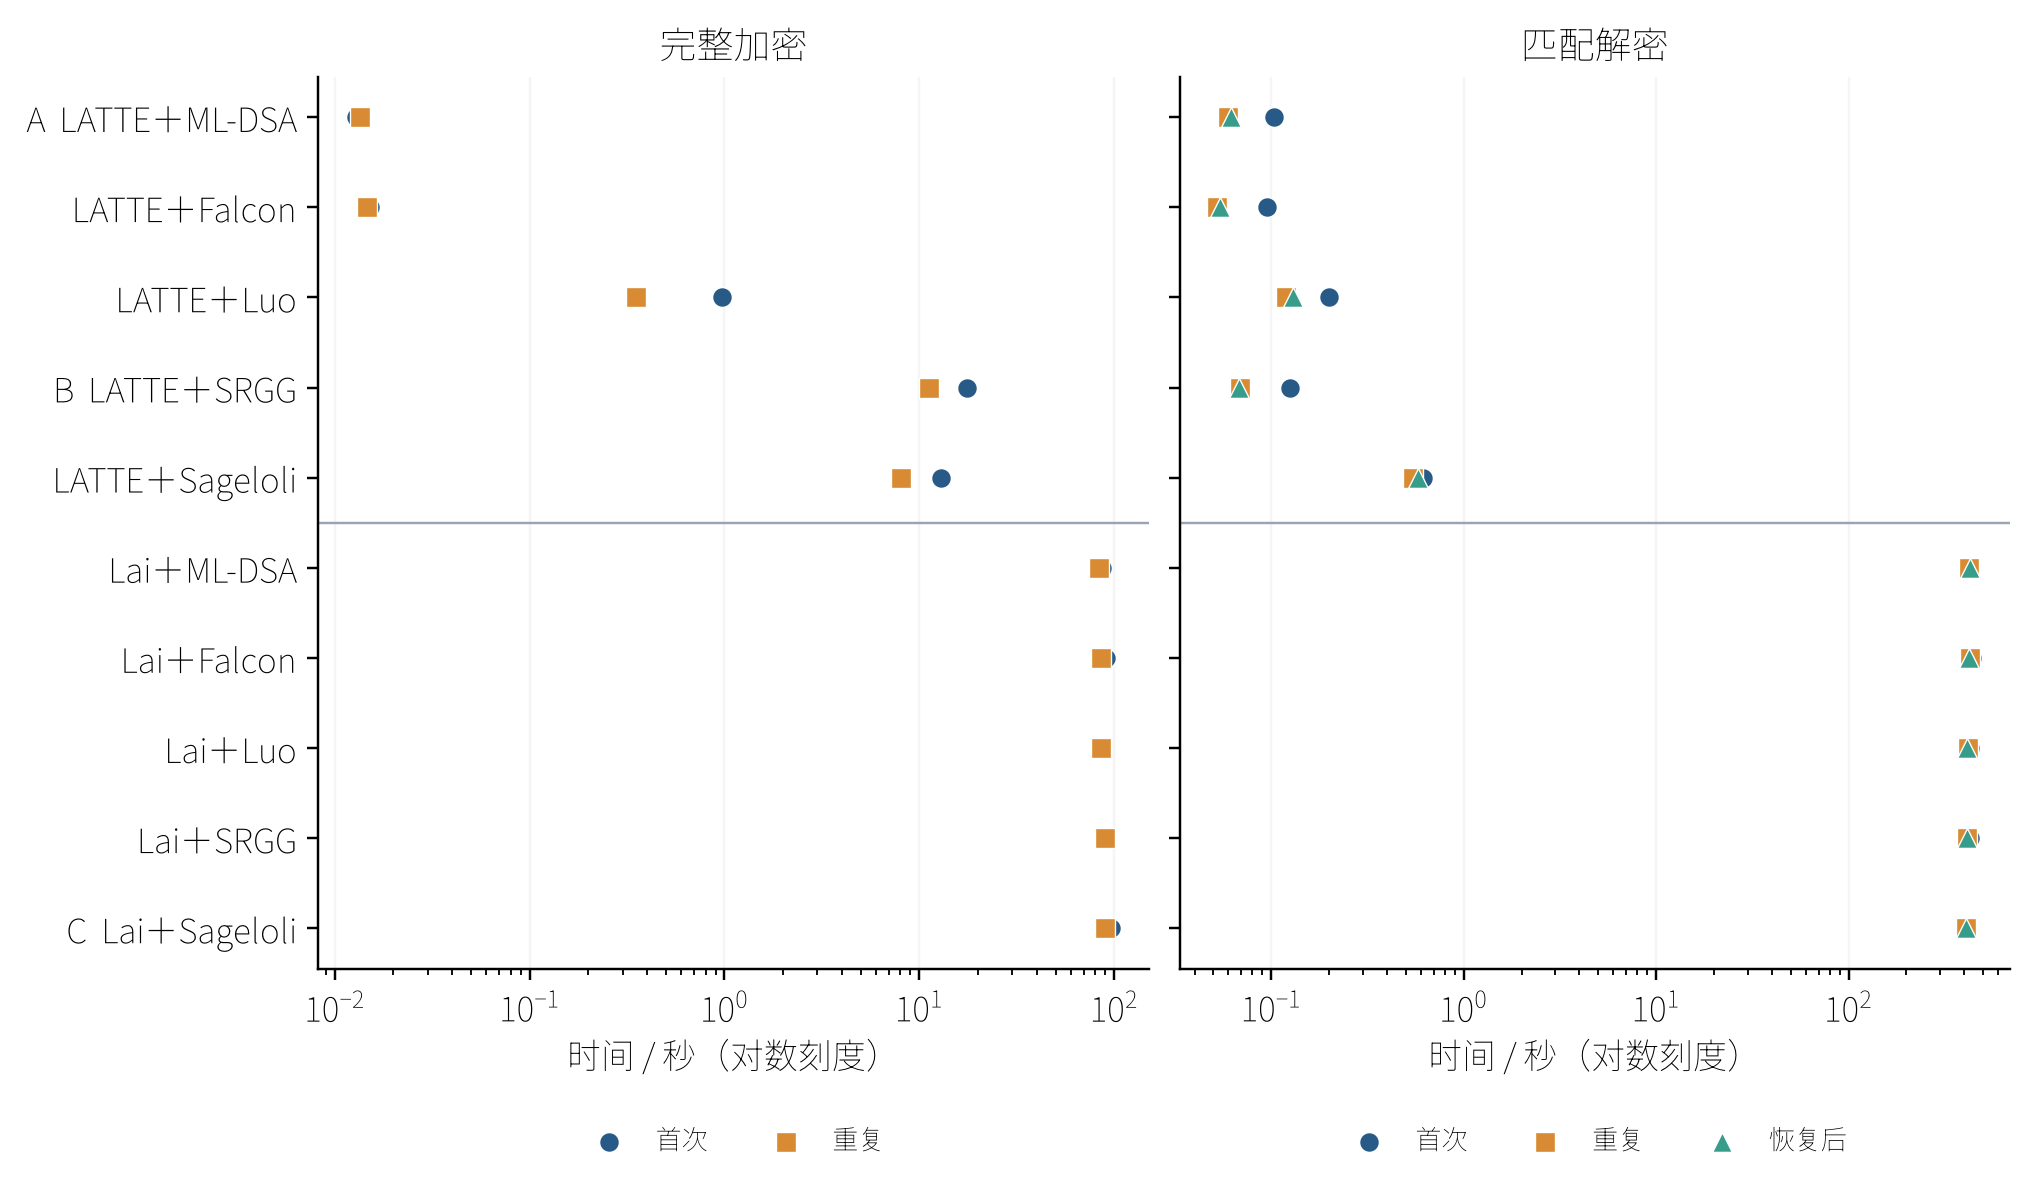
\includegraphics[width=.98\textwidth]{figures/ten-combination-times.png}
\caption{十种组合的首次、重复与恢复后完整操作时间；A、B、C为三组代表}
\label{fig:ten-combination-times}
\end{figure}

LATTE＋Luo、SRGG和Sageloli的重复加密分别降至0.351、11.3和8.04秒，与相同发送密钥下可以
复用部分数值准备的实现结构一致。LATTE五组恢复后解密为54.5至577毫秒，和同进程重复解密接近，
说明规范对象加载没有改变接收路径的量级。Lai五组恢复后解密仍为406至428秒，因为恢复不会缓存
新的随机委派结果；这与第五章另行讨论的“准备接收会话”是两种不同状态策略。

\subsection{规范对象尺寸与运行内存}

表~\ref{tab:ten-object-sizes}列出同一系统根产生的公共对象、主状态、双方角色对象和完整密文。
尺寸均取实际规范二进制编码长度，不使用数学对象的内存估算。

\begin{table}[H]
\centering\small
\caption{十种组合的规范对象与完整密文长度}
\label{tab:ten-object-sizes}
\setlength{\tabcolsep}{3.2pt}
\begin{tabular}{@{}lrrrrr@{}}
\toprule
\rowcolor{black!8} 组合 & 公共对象 & 主状态 & 发送钥 & 接收状态 & 完整密文 \\
\midrule
% BEGIN DATA ten-object-sizes.tex
LATTE＋ML-DSA & 14.1~KiB & 142~KiB & 7.86~KiB & 125~KiB & 139~KiB \\
LATTE＋Falcon & 13.7~KiB & 137~KiB & 4.1~KiB & 125~KiB & 135~KiB \\
LATTE＋Luo & 255~KiB & 479~KiB & 306~KiB & 125~KiB & 148~KiB \\
LATTE＋SRGG & 46.2~KiB & 231~KiB & 82.4~KiB & 125~KiB & 146~KiB \\
LATTE＋Sageloli & 3.36~MiB & 149~MiB & 137~MiB & 125~KiB & 3.21~MiB \\
Lai＋ML-DSA & 1.54~MiB & 3.86~MiB & 7.86~KiB & 19.5~MiB & 1.27~MiB \\
Lai＋Falcon & 1.54~MiB & 3.85~MiB & 4.1~KiB & 19.5~MiB & 1.27~MiB \\
Lai＋Luo & 1.78~MiB & 4.19~MiB & 306~KiB & 19.5~MiB & 1.28~MiB \\
Lai＋SRGG & 1.58~MiB & 3.95~MiB & 82.3~KiB & 19.5~MiB & 1.28~MiB \\
Lai＋Sageloli & 4.9~MiB & 153~MiB & 137~MiB & 19.5~MiB & 4.34~MiB \\
% END DATA ten-object-sizes.tex
\bottomrule
\end{tabular}
\end{table}

接收状态几乎完全由HIBE决定：LATTE五组约为125~KiB，Lai五组约为19.5~MiB。发送钥则主要由
IBS决定，同一种IBS分别搭配两种HIBE时长度基本一致。完整密文也呈现可分解的结构：固定IBS后，
由LATTE换为Lai会增加约1.137~MiB；采用Sageloli时，大型IBS签名又使完整密文达到3.21和
4.34~MiB。该规律与后文按字段核算密文组成的结果一致。

图~\ref{fig:ten-combination-resources}把完整密文与运行期间的最大采样RSS并列。除Sageloli外，
十种组合各阶段最大采样RSS约为254至885~MiB；LATTE＋Sageloli约1.64~GiB，Lai＋Sageloli约
1.97~GiB。RSS每10毫秒采样一次，包含运行库与子进程，共享页可能重复计数，因而用于同批次资源
比较；它记录的是进程树采样值，并非物理页的精确分解。

\begin{figure}[H]
\centering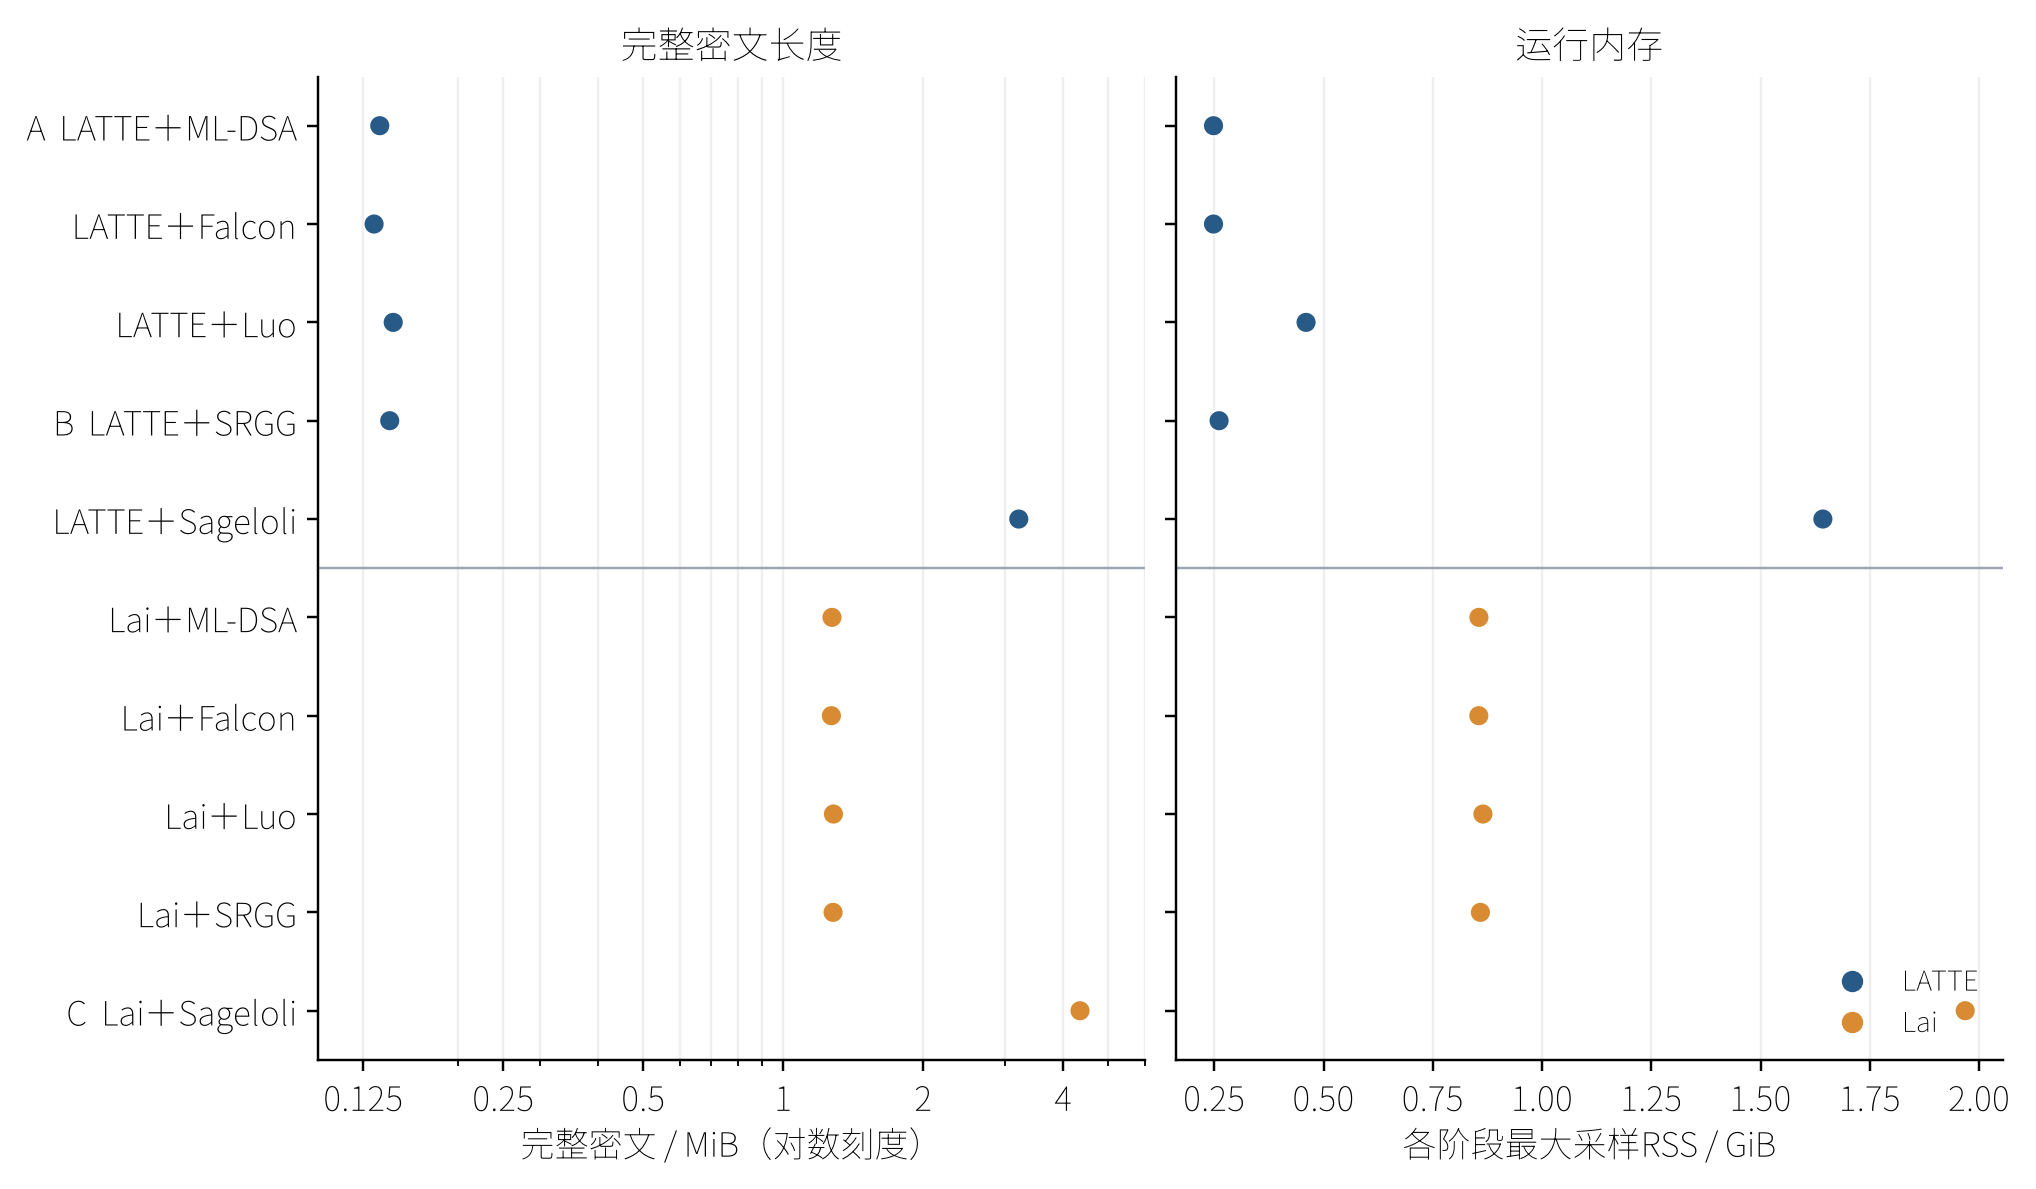
\includegraphics[width=.98\textwidth]{figures/ten-combination-resources.png}
\caption{十种组合的完整密文长度与各阶段最大进程树采样RSS}
\label{fig:ten-combination-resources}
\end{figure}

\subsection{组合差异与代表方案}

横向结果表明，HIBE和IBS影响完整系统的不同位置。HIBE主要决定接收状态、HIBE胶囊和解密委派；
IBS主要决定发送者发钥、签名生成、发送钥和签名字段。采用LATTE时，五种IBS的发送差异可以直接
观察；采用Lai时，HIBE成本占主导，但不同IBS仍通过密钥和密文长度体现。因而系统选型不宜把全部
指标压缩成单一总分，而应分别考虑发钥机构、发送端、接收端和网络侧资源。

三组代表由此对应三种明确用途。A提供低延迟标准化签名路径；B保留快速接收，同时展示原生模格
IBS和紧凑编码的发送端代价；C覆盖另一HIBE与环格IBS，并为结构化采样和固定身份对会话优化提供
完整对象。第四章的代表方案表采用本节同机数据；下面的多根与阶段实验进一步分析运行波动和
瓶颈组成。

\section{代表方案的重复与专项分析}
专项实验用于分析运行波动、单项优化和内部阶段，所用机器、输入与重复方式列于表
~\ref{tab:specialized-environments}。这些数据按各自实验条件单独呈现；表~\ref{tab:environments}
中的十种组合单根实测继续作为统一横向比较。

\begin{table}[H]
\centering\small
\caption{代表方案与优化专项实验的环境及用途}
\label{tab:specialized-environments}
\begin{tabularx}{\textwidth}{@{}>{\raggedright\arraybackslash}p{.18\textwidth}>{\raggedright\arraybackslash}p{.34\textwidth}>{\raggedright\arraybackslash}X@{}}
\toprule
\rowcolor{black!8} 实验 & 环境 & 输入、重复与用途 \\
\midrule
A/B多根重复 & i9-14900HX，Sage 10.7／Python 3.12.13 & 每组3个独立根，每根3对重复操作；观察根间与根内波动 \\
Sageloli采样 & Ultra 7 255HX，Python 3.13.15 & PARAM-I、II各1套；测量结构化发钥、签名和验证 \\
SRGG编码 & Ultra 7 255HX，Python 3.13.15 & 每档3套；同一对象两种格式各交替测量5次 \\
C阶段分解 & Ultra 9 275HX，Sage 10.9／Python 3.13.14 & C组合1次，分解委派与后续阶段 \\
Lai接收会话 & i9-14900HX，Sage 10.7／Python 3.12.13 & 1套系统；原路径2次、准备1次、会话内解密3次 \\
部署位置 & Ultra 9 275HX，Python 3.13.14 & 相同3套状态；每种位置各30次加密和解密 \\
\bottomrule
\end{tabularx}
\end{table}

\subsection{A/B多根重复实验}
A、B使用相同LATTE参数与相同输入，主要差别在IBS。该批实验在另一台机器上分别建立3个独立
系统根，每根执行3次重复操作，用于观察固定组合的运行波动。表~\ref{tab:ab-times}给出完整生命
周期的中位时间，图~\ref{fig:ab-times}展示重复加解密的9次观测。该批结果用于补充多根运行波动，
前述单根同机结果用于组合间横向比较。

\begin{table}[H]
\centering\small
\caption{A/B完整流程中位时间，单位为秒}
\label{tab:ab-times}
\begin{tabular}{@{}lrrr@{}}
\toprule
\rowcolor{black!8} 操作 & A & B & 测量次数（A/B） \\
\midrule
% BEGIN DATA ab-timings.tex
系统建立 & 1.12 & 1.6 & 3/3 \\
发送者发钥 & 0.0954 & 32.1 & 3/3 \\
接收者发钥 & 0.427 & 0.457 & 3/3 \\
首次加密 & 0.0963 & 9.14 & 3/3 \\
首次解密 & 0.284 & 0.239 & 3/3 \\
重复加密 & 0.0785 & 9.17 & 9/9 \\
重复解密 & 0.152 & 0.161 & 9/9 \\
对象恢复 & 0.845 & 0.89 & 3/3 \\
恢复后解密 & 0.154 & 0.134 & 9/9 \\
% END DATA ab-timings.tex
\bottomrule
\end{tabular}
\end{table}

两组接收者发钥和重复解密接近，额外成本主要出现在B的发送者发钥与签名生成。A、B重复加密中位数分别为78.5毫秒和9.17秒，重复解密分别为152毫秒和161毫秒。A适合作为交互演示基线；B展示原生模块格IBS在同一完整协议中的运行特点。

\begin{figure}[H]
\centering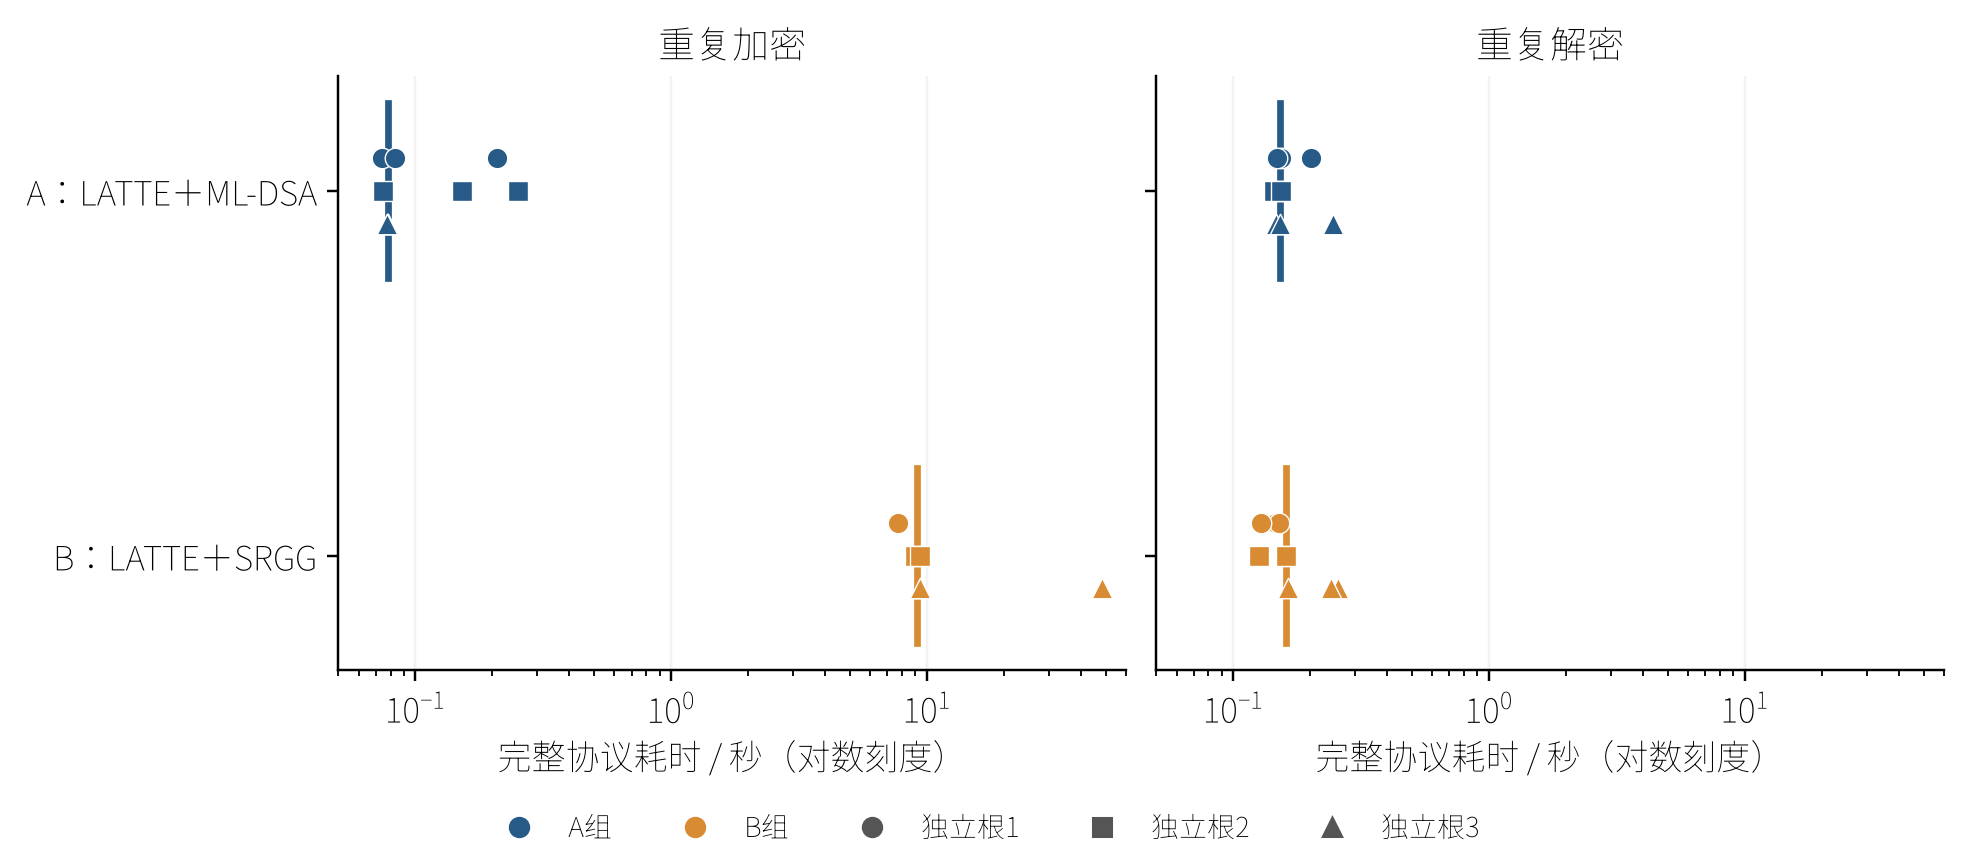
\includegraphics[width=.98\textwidth]{figures/ab-times.png}
\caption{A/B重复加密与解密的9次观测；点形区分三个独立根，短竖线标出各组中位数，横轴采用对数刻度}
\label{fig:ab-times}
\end{figure}

全部观测显示，B有一次重复加密耗时约48.2秒，明显高于其中位数；A也有较慢观测。首次解密包含
叶钥生成，因此通常高于重复解密；恢复对象后，解密回到与重复操作相近的量级。

\subsection{A/B多根实验的对象尺寸与内存}
表~\ref{tab:ab-sizes}汇总公共对象、主状态和双方密钥的编码长度。A、B完整密文约139 KiB和146 KiB；本章后面的密文组成分析进一步解释这些字节来自哪里。

\begin{table}[H]
\centering\small
\caption{A/B对象编码长度约值与运行内存}
\label{tab:ab-sizes}
\begin{tabular}{@{}crrrrrr@{}}
\toprule
\rowcolor{black!8} 组 & 公钥 & 主状态 & 发送钥 & 接收状态 & 完整密文 & 内存/MiB \\
\midrule
% BEGIN DATA ab-sizes.tex
A & 14 & 173 & 7.86 & 125 & 139 & 460 \\
B & 46.2 & 262 & 82.4 & 125 & 146 & 485 \\
% END DATA ab-sizes.tex
\bottomrule
\end{tabular}
\begin{minipage}{.96\textwidth}\footnotesize
前五项单位为KiB。对象长度按记录范围取近似值；内存为每10毫秒采样的进程树RSS最高值，包含运行库和子进程，短时峰值可能未被采样捕获。
\end{minipage}
\end{table}

B的公钥、主状态与发送钥大于A，接收状态接近，符合两组共用HIBE而采用不同IBS的结构。编码文件大小和运行内存分别统计：紧凑密钥文件加载后仍会恢复为数学对象，运行时还需要数值库、采样工作区和子进程。

\subsection{C组合的委派开销}
十种组合的主实验中，C的首次加密和解密分别为96.4秒和412秒。另一次保存了内部阶段的32字节消息
测试记录：加密99.0秒，匹配解密425秒，其中Lai委派为393秒，占约92.5\%。两次运行的条件和
用途分别为完整运行和内部阶段分析，两份记录都表明接收端的主要瓶颈是为认可发送身份生成叶钥。该阶段分解
记录的解密进程存在并发，因此只用于说明成本组成。

C的传输密文约4.34 MiB，大部分来自Sageloli签名和Lai胶囊。它展示了另一类HIBE与环IBS在论文配置下的完整组合，以及会话摊销的使用方式。下面分别分析通信量与准备成本。

\subsection{Wang--PW目标档的分阶段运行}

Wang--PW目标档使用$n=512$、$q=4294967291$和$s_0=4$。其密钥和采样工作区远大于常规组合，
因此在128~GiB级服务器上完成目标规模运行。表~\ref{tab:wang-results}汇总已经保存的建立、发钥、
独立签名和LATTE组合结果。

\begin{table}[H]
\centering\small
\caption{Wang--PW目标档与LATTE组合的实测结果}
\label{tab:wang-results}
\begin{tabularx}{\textwidth}{@{}p{.28\textwidth}rX@{}}
\toprule
\rowcolor{black!8} 项目 & 结果 & 说明 \\
\midrule
Setup & 536.63 s & 生成目标档公开矩阵和根陷门 \\
公开参数 & 67,109,371 B & 规范二进制对象 \\
主状态 & 603,980,295 B & 保存紧凑根陷门与参数 \\
KeyExtract & 5,431.95 s & 为一个64字节身份生成用户陷门 \\
用户签名密钥 & 2,214,593,131 B & 规范二进制对象 \\
独立Sign & 175.79 s、175.15 s & 两次恢复后的新消息签名均通过公开验签 \\
签名 & 393,320 B & 包含身份盐、消息盐和短原像 \\
签名峰值RSS & 约41.3 GiB & 进程树采样峰值 \\
LATTE＋Wang加密 & 192.54 s & 78字节应用消息，包含一次新Wang签名 \\
匹配解密 & 2.85 s & 从恢复的接收状态完成诚实解密 \\
完整密文 & 529,207 B & Hybrid与完整字节认证后的wire长度 \\
组合驱动总时长 & 254.86 s & 含准备、一次加密、诚实解密和错误输入检查 \\
\bottomrule
\end{tabularx}
\end{table}

目标档实验分阶段保存并复用已经生成的根和用户密钥。Setup、KeyExtract来自较早的目标生命周期，
最终两次签名与LATTE组合使用修订后的签名实现；表中按阶段独立呈现各项结果。

从使用过程看，Setup和KeyExtract适合放在发钥机构的离线阶段。发送端一次签名约176秒，并需要
约41.3~GiB峰值内存，是组合加密的主要成本。接收端只进行公开验签与LATTE解封装，诚实解密约
2.85秒。393,320字节IBS签名进入对称载荷后，完整密文约517~KiB，明显小于用户签名密钥，
但仍高于A、B。

这一结果表明通用框架能够容纳大对象矩阵SIS后端，同时也说明它更适合低频签名、离线发钥和
资源充足的发送端。三组代表保持A、B、C不变，Wang--PW作为目标规模补充方案单独展示。

\section{完整密文的通信开销}
\subsection{完整密文的组成}
混合加密使应用消息不再受HIBE短明文容量直接限制，但种子胶囊、IBS签名和一次性认证仍需要传输。依据现有安装运行记录与实际编码格式，可将A的一条32字节消息和C的一条空消息分解为表~\ref{tab:ciphertext-parts}。

\begin{table}[H]
\centering\small
\caption{两条已有密文的字节组成核算}
\label{tab:ciphertext-parts}
\begin{tabular}{@{}lrr@{}}
\toprule
\rowcolor{black!8} 组成部分 & A：消息32 B & C：空消息 \\
\midrule
一次性公钥 & 65,536 & 65,536 \\
一次性签名 & 32,768 & 32,768 \\
IBS签名 & 6,237 & 3,227,824 \\
HIBE胶囊 & 37,088 & 1,228,844 \\
应用消息 & 32 & 0 \\
上下文、格式、nonce与标签 & 432 & 432 \\
\midrule
合计 & 142,093 & 4,555,404 \\
\bottomrule
\end{tabular}
\begin{minipage}{.96\textwidth}\footnotesize
整包长度来自已有运行；固定字段按序列化模块核算，HIBE胶囊长度由整包扣除其他组成得到。该核算没有新增加密实验。
\end{minipage}
\end{table}

\begin{figure}[H]
\centering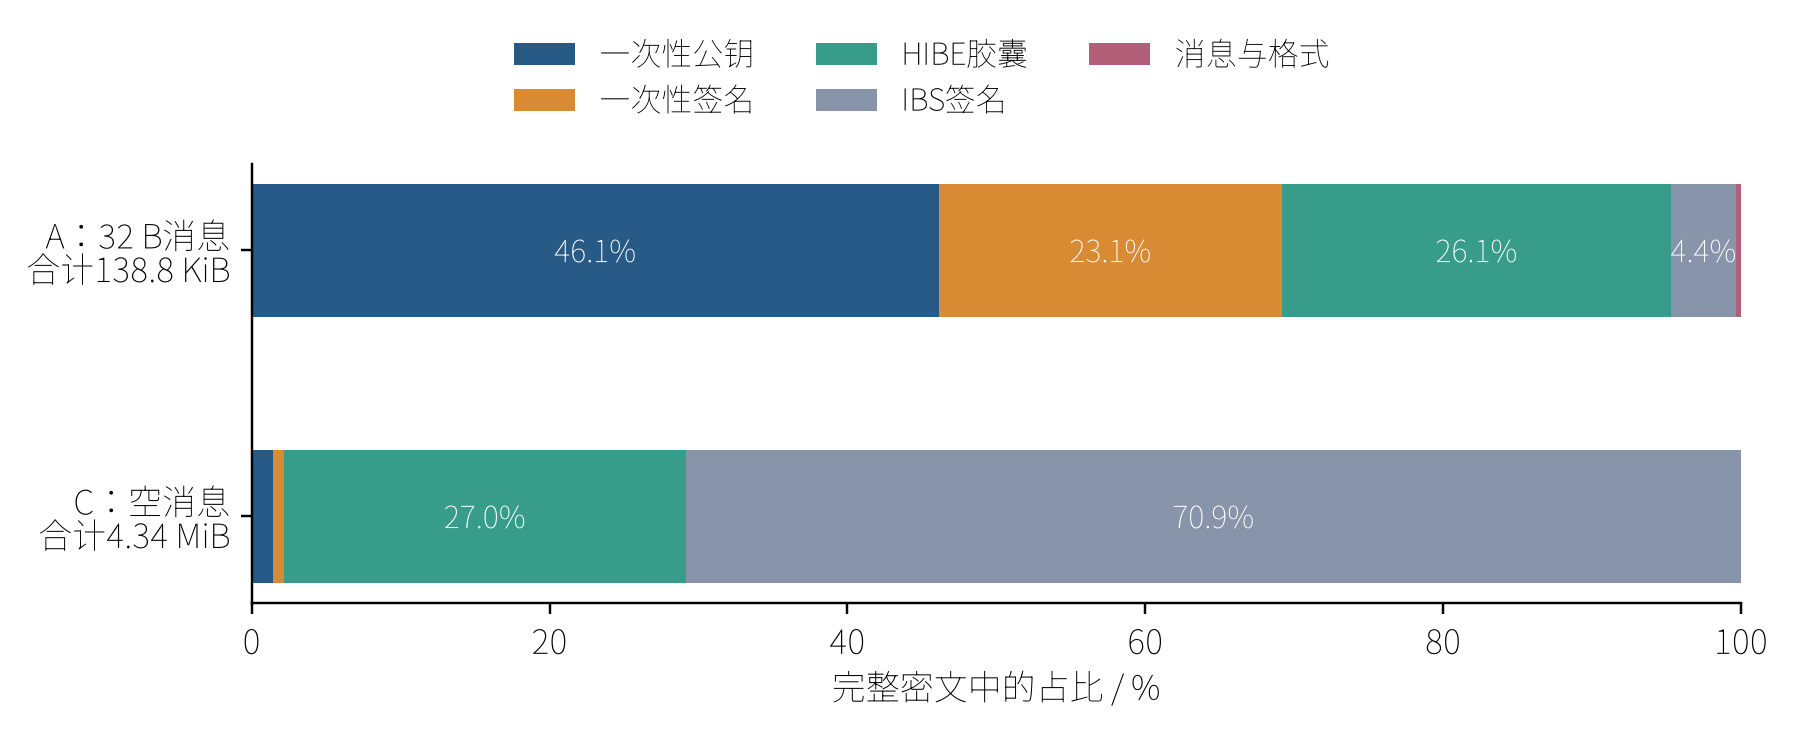
\includegraphics[width=.98\textwidth]{figures/ciphertext-parts.png}
\caption{完整密文的主要成本来源：A以一次性认证为主，C以IBS签名和HIBE胶囊为主}
\label{fig:ciphertext-parts}
\end{figure}

Lamport一次性公钥含1,024个64字节哈希像，签名含512个64字节原像，两项合计固定96 KiB，约占这条A密文的69.2\%。因此，缩短几字节应用消息几乎不会改变A的整包长度。C的IBS签名约占70.9\%，HIBE胶囊约占27.0\%；其后续通信优化应优先考察这两部分。

这也解释了SRGG签名紧凑编码与完整B密文的关系：签名字段变短会减少对称载荷，但整包还包含与A相同的一次性认证结构和LATTE胶囊。评价编码时应同时看单体对象与完整协议中的占比。

\subsection{消息长度与可用容量}
安装运行测试已完成A的0、32、1,024和59,191字节消息，B的0、32、1,024和65,364字节消息；超过应用上限1字节时，系统在生成新密文前拒绝。该批最大长度密文约为197 KiB和210 KiB。

C已完成空消息和1,024字节消息，两条密文相差1,024字节，符合固定胶囊与签名加上可变应用载荷的组成。C的3,924字节上限来自容量计算，尚缺该最大长度的加密解密记录。上述容量检查使用签名保守上界，具体签名和胶囊的编码长度仍可能随随机输出变化。

\section{三项主要优化的实验结果}
\subsection{Sageloli结构化采样结果}
Sageloli两个参数档均完成建立、身份发钥、两次签名和验证。表~\ref{tab:sageloli-times}给出各档一套系统的运行记录。

\begin{table}[H]
\centering\small
\caption{Sageloli结构化实现的实际运行，时间单位为秒}
\label{tab:sageloli-times}
\begin{tabular}{@{}lrrrrrr@{}}
\toprule
\rowcolor{black!8} 参数档 & 建立 & 发钥 & 首次签名 & 后续签名 & 验证 & RSS/GiB \\
\midrule
% BEGIN DATA sageloli-times.tex
PARAM-I & 4.99 & 85.1 & 9.28 & 2.02 & 0.517 & 1.36 \\
PARAM-II & 43.6 & 520 & 38.6 & 5.02 & 1.36 & 6.19 \\
% END DATA sageloli-times.tex
\bottomrule
\end{tabular}
\end{table}

PARAM-I发钥约85.1秒，记录峰值RSS约1.36 GiB；PARAM-II发钥约520秒，约6.19 GiB。首次签名
明显高于第二次，与同一身份陷门下数值计划可以复用的实现结构相符。两档参数都完成采样和公开
验证。第五章的1.18~TiB是稠密矩阵表示的理论存储量估算，本表记录的是未展开该矩阵的结构化
实现，因此二者分别说明原始瓶颈与实际资源占用。

\Needspace{.45\textheight}
\subsection{SRGG紧凑编码结果}
图~\ref{fig:codec}和表~\ref{tab:codec-sizes}展示三档SRGG相同数学对象的两种编码。每档独立建立3套系统，在同一对象上交替执行两种格式的编解码。

\begin{figure}[H]
\centering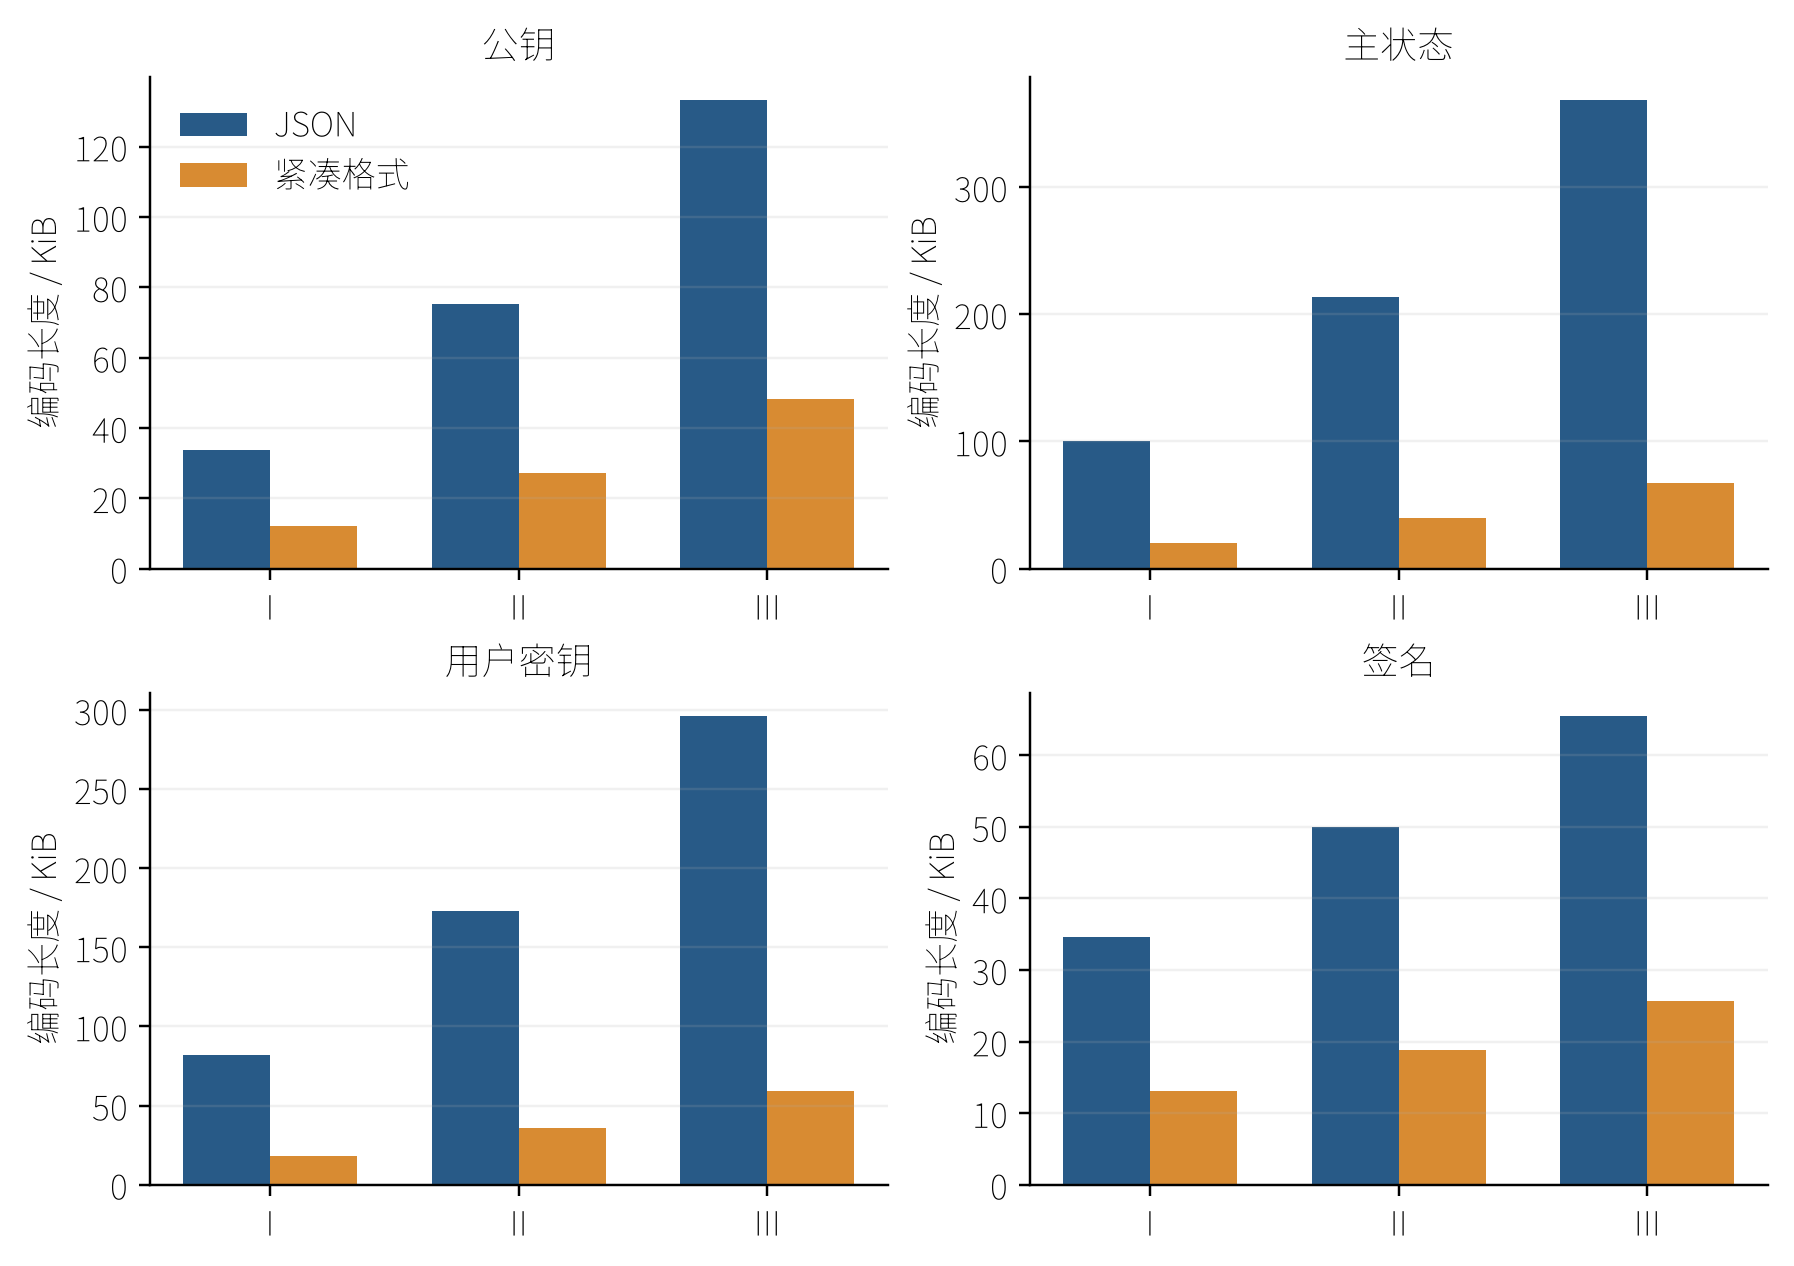
\includegraphics[width=.96\textwidth]{figures/codec.png}
\caption{SRGG三档参数的四类对象尺寸；I、II、III表示参数档}
\label{fig:codec}
\end{figure}

\begin{table}[H]
\centering\small
\caption{SRGG对象编码长度，单位为KiB}
\label{tab:codec-sizes}
\begin{tabular}{@{}lrrrr@{}}
\toprule
\rowcolor{black!8} 参数档／格式 & 公钥 & 主状态 & 用户钥 & 签名 \\
\midrule
% BEGIN DATA codec-sizes.tex
I／JSON & 33.7 & 100 & 82.2 & 34.5 \\
I／紧凑 & 12.1 & 19.8 & 17.8 & 13.1 \\
II／JSON & 75.2 & 213 & 173 & 49.9 \\
II／紧凑 & 27.1 & 40.1 & 35.6 & 18.8 \\
III／JSON & 133 & 368 & 296 & 65.5 \\
III／紧凑 & 48.1 & 67.5 & 59.5 & 25.6 \\
% END DATA codec-sizes.tex
\bottomrule
\end{tabular}
\end{table}

紧凑格式下，公钥占相应JSON长度的35.9\%至36.2\%，主状态占18.3\%至19.8\%，用户密钥占
20.1\%至21.7\%，签名占37.7\%至39.1\%。主状态中小范围陷门系数所占比例较高，按实际取值
范围位打包后，长度降幅最明显。

空间收益伴随位打包和规范检查的时间成本。以PARAM-I主状态为例，紧凑编码、解码中位时间约为
23.1毫秒和61.3毫秒，JSON编码、解码约为0.974毫秒和37.3毫秒。对于主状态保存、角色密钥
传递和签名传输，长度下降带来的收益更直接；高频内存内转换则需要同时考虑额外处理时间。

\subsection{Lai接收会话结果}
Lai会话实验使用一套主密钥，原路径解密2次，建立会话1次，会话内解密3次。原解密中位数为526秒，会话准备约510秒，后续解密中位数为28.6秒；叶钥编码长度为34.7~MiB。

\begin{figure}[H]
\centering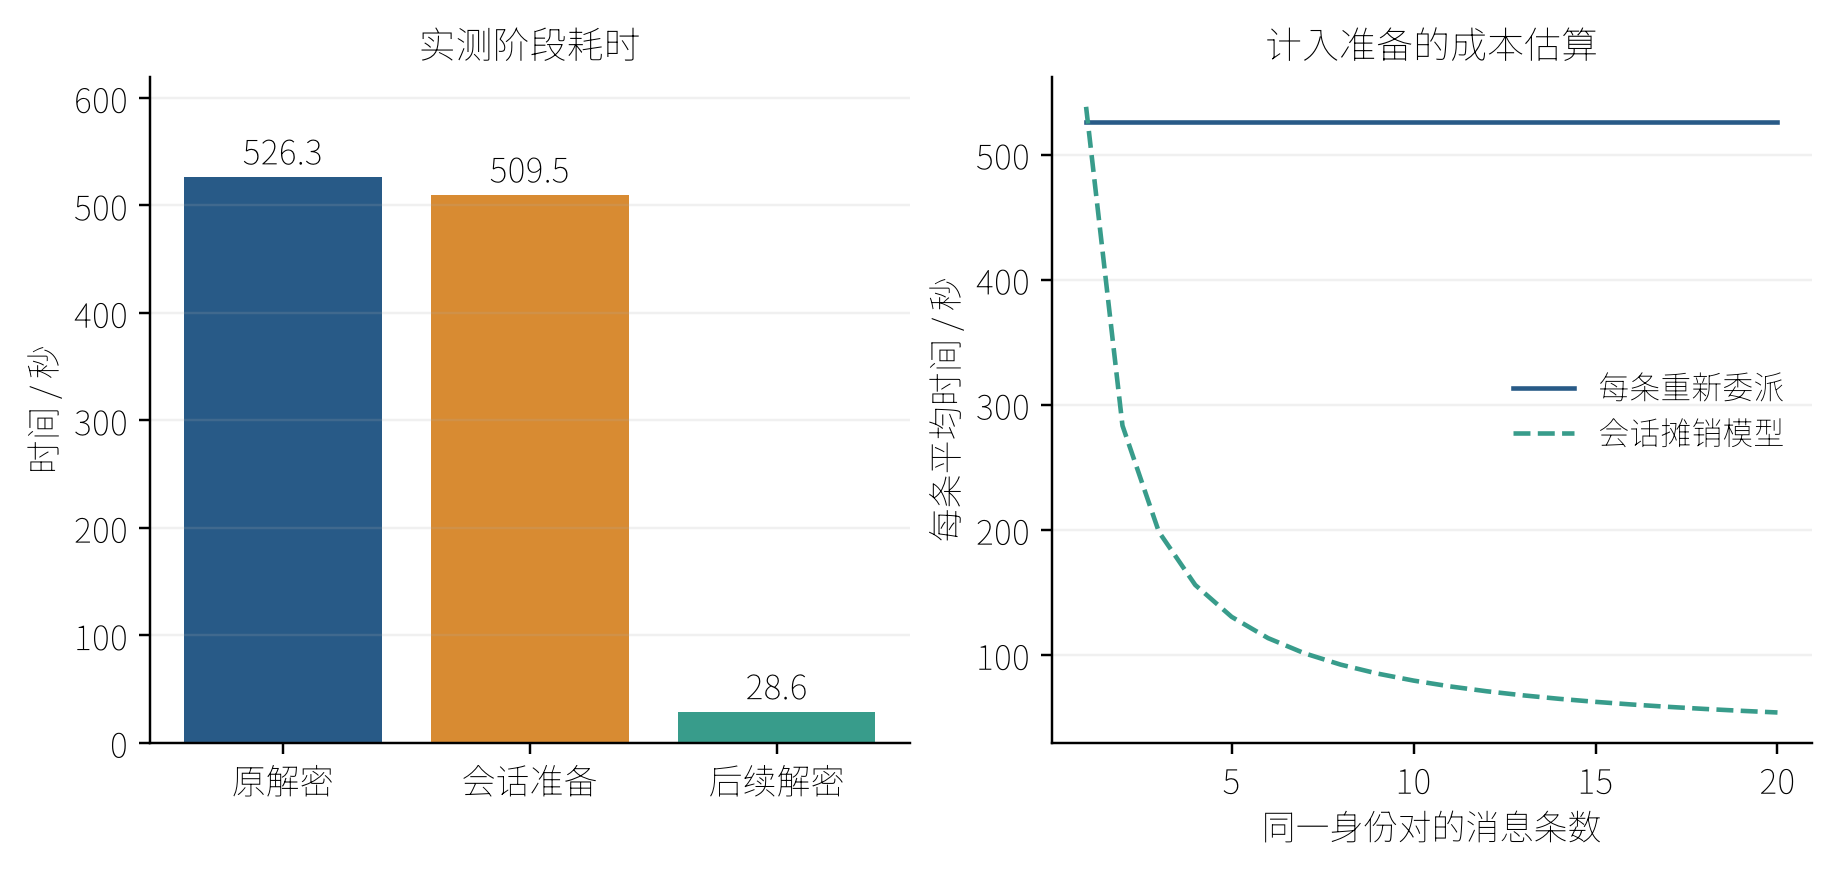
\includegraphics[width=.98\textwidth]{figures/session.png}
\caption{Lai接收会话：左图为测得阶段耗时，右图由阶段中位数代入成本公式估算}
\label{fig:session}
\end{figure}

准备完成后的单条时间约为原路径的$1/18.4$。把准备计入后，首条平均成本约538秒；按$\bar T(N)$模型，处理10条和100条消息时约为79.5秒和33.7秒。累计成本临界式给出$N>1.024$，因此从第2条消息起，会话模型的累计时间低于逐条委派。右图是将已有阶段中位时间代入成本公式得到的模型曲线。

会话方法把主要委派开销移到首次使用，适合固定身份对的连续消息。短暂的一次通信仍要承担完整准备；长期会话则以额外秘密状态换取较低的后续延迟。该组样本来自一套系统，后续扩大测量可进一步观察不同主密钥下的波动。

\section{缓存与部署位置的完整流程对照}
\subsection{局部缓存对总耗时的影响}
在A、B各3套系统中，分别开启和关闭优化，以相同输入执行完整流程。A缓存机构证书的成功验证结果，原生验签调用由每条2次减少为1次，解密时间比中位数为1.086，逐套范围0.992至1.339。B复用签名数值准备，加密时间比中位数1.030，范围1.009至1.921。

这些结果说明，减少一次局部调用后，总时间仍受其余密码运算与运行波动影响。A有一套测量略微回退，B的中位收益较小。因此，系统保留缓存容量与关闭选项，主要优化结论仍以结构表示、编码和Lai会话为重点。

\subsection{文件部署位置对运行时间的影响}
三路部署对照固定参数、状态和原生引擎，均由同一WSL Python运行，分别使用Windows盘源码、Windows盘安装包及Linux盘同一安装包。每路完成30次完整加密和30次解密，图~\ref{fig:placement}给出中位数。

\begin{figure}[H]
\centering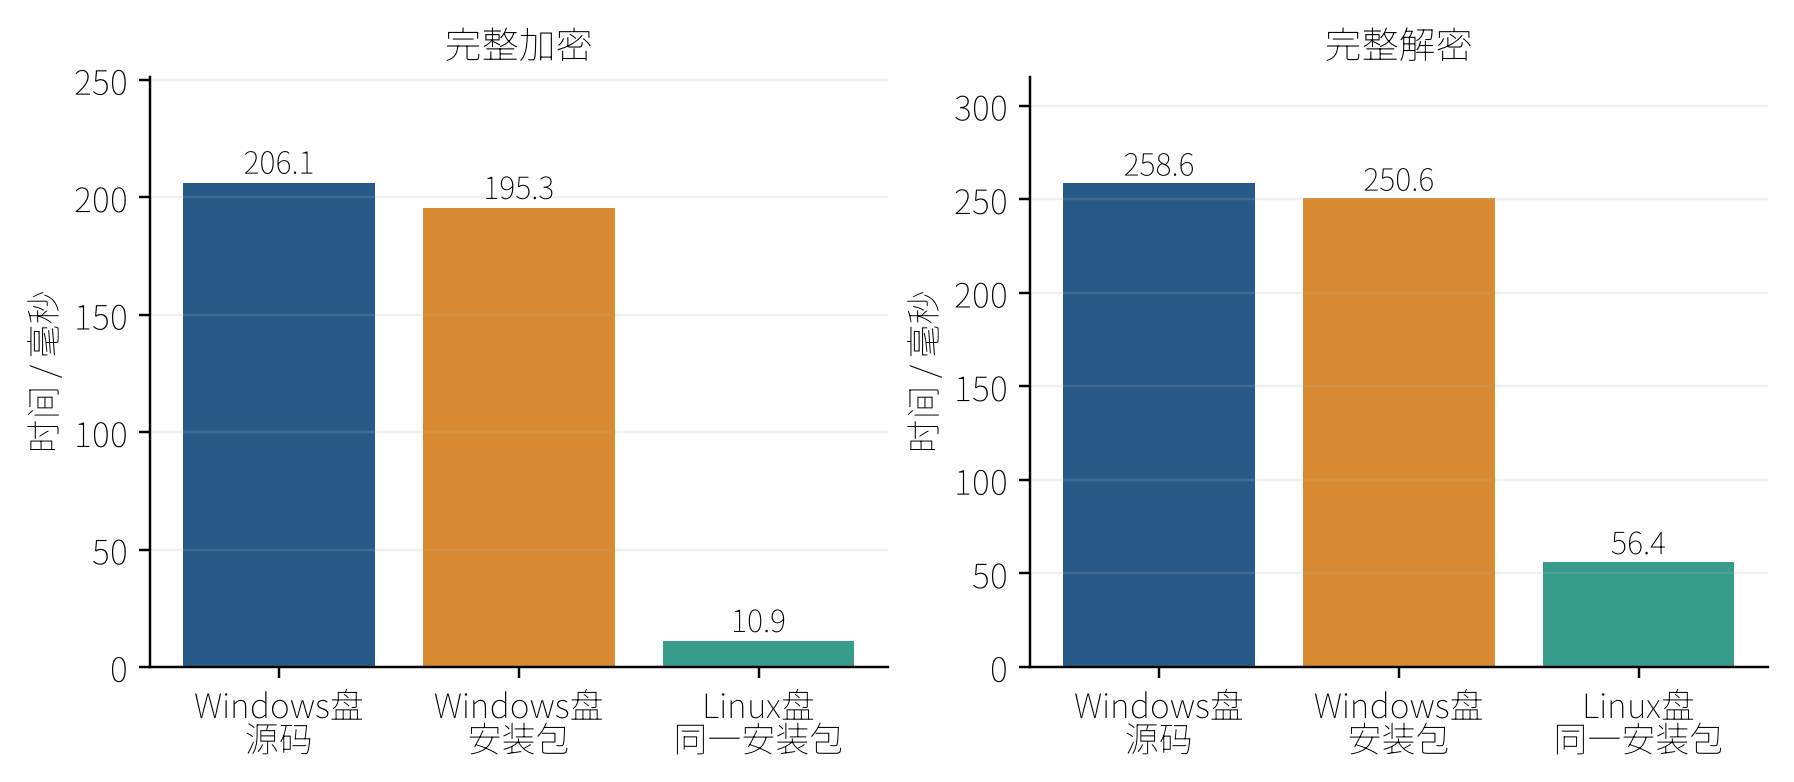
\includegraphics[width=.98\textwidth]{figures/placement.png}
\caption{文件放置位置对完整A流程的影响；三路均使用同一WSL运行时}
\label{fig:placement}
\end{figure}

Linux本地安装包的加密、解密中位时间分别为Windows盘源码运行的5.30\%和21.8\%。排除源码与
安装包差异，只比较同一安装包的两种位置时，相应比例为5.59\%和22.5\%。剖析记录中，5次加密
产生的515次文件读取在挂载目录累计约1.073秒，在Linux本地约0.011秒，说明文件访问是该批
运行的重要成本。因此，WSL部署优先把安装包和运行状态置于Linux本地文件系统。

\section{功能测试结果}
十种组合的同机实验中，每组均通过2次诚实加密、3次诚实解密、1次新进程恢复，以及截断和单比特
翻转两项外层拒绝，合计20次加密、30次解密、10次恢复和20次拒绝。更完整的异常语义由三组
代表实验覆盖：三组均完成双方匹配恢复、三类身份错配和多种字节异常拒绝。表
~\ref{tab:functional}汇总主要检查；另有A的随机身份与消息批次，独立建立3套系统、测试12组输入，
60/60项判断符合预期。

\begin{table}[H]
\centering\small
\caption{三组完整协议的主要功能结果}
\label{tab:functional}
\begin{tabularx}{\textwidth}{@{}Xccc@{}}
\toprule
\rowcolor{black!8} 检查情况 & A & B & C \\
\midrule
双方身份匹配 & 恢复原文 & 恢复原文 & 恢复原文 \\
仅接收身份不匹配 & 拒绝 & 拒绝 & 拒绝 \\
仅期望发送身份不匹配 & 拒绝 & 拒绝 & 拒绝 \\
双方身份都不匹配 & 拒绝 & 拒绝 & 拒绝 \\
密文字节修改、截断、追加或重复字段 & 拒绝 & 拒绝 & 拒绝 \\
外层认证有效、内部签名无效 & 拒绝 & 拒绝 & 拒绝 \\
新进程加载对象后解密 & 成功 & 成功 & 成功 \\
\bottomrule
\end{tabularx}
\end{table}

身份错配测试覆盖接收者、发送者和双方同时错误，分别触发不同层次的拒绝。密文字节修改、截断、
追加和重复字段覆盖外层认证与规范解析；“外层认证有效、内部签名无效”则单独检查IBS身份认证。
新进程恢复测试重新加载公开对象和角色密钥，再对已有密文解密，覆盖持久对象的完整使用路径。

\section{本章小结}

十种常规组合在统一机器、输入和运行配置下全部完成。横向结果表明，HIBE主要决定接收状态、胶囊
长度和解密委派，IBS主要决定发送者发钥、签名生成和发送钥尺寸。A的在线收发处于毫秒级；B的
主要时间集中在发送端SRGG签名，接收端仍为亚秒级；C的主要时间集中在Lai叶钥委派。Wang--PW
的Setup、发钥和签名需要服务器级资源，但接收端解密保持在数秒量级。

通信量分析表明，A的密文主要由一次性认证构成，C主要由IBS签名和HIBE胶囊构成。对象级优化
能否明显缩短完整密文，取决于目标字段在整包中的占比。功能测试与恢复测试进一步确认，同一套
协议在A、B、C以及十种常规组合中保持一致的身份匹配和字节处理流程。三项主要优化分别降低了
Sageloli采样内存、SRGG对象尺寸和Lai连续解密延迟。
